Når man f.eks. lager transistorer bruker man dopa halvledere.
\\\\
Halvledere som karbon, silisium og germanium har 4 valenselektroner
som etter oktettregelen danner kovalente bindinger.
\marginpar{oktettregelen:
atomer "ønsker" å binde seg til hverandre s.a. de får 8 valenselektroner}
\\\\
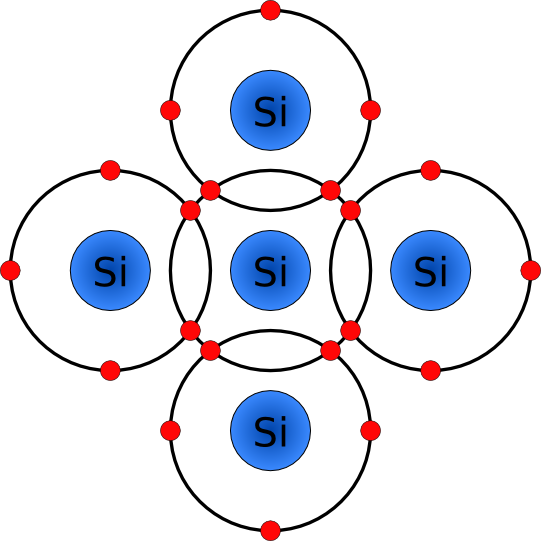
\includegraphics[width=0.5\textwidth]{./img/kovalent-Si}
\\
Silisium atomer i diamantstruktur



\subsubsection{n-type}
For å dope et stoff som ovenfor,
tilsetter man atomer med 3 eller 5 valenselektroner.
\\\\
I n-type doping tilsettes atomer med 5 valenselektroner.
Slike atomer kalles donor-atomer,
da man får et ekstra elektron som kan flyte rundt.
\\\\
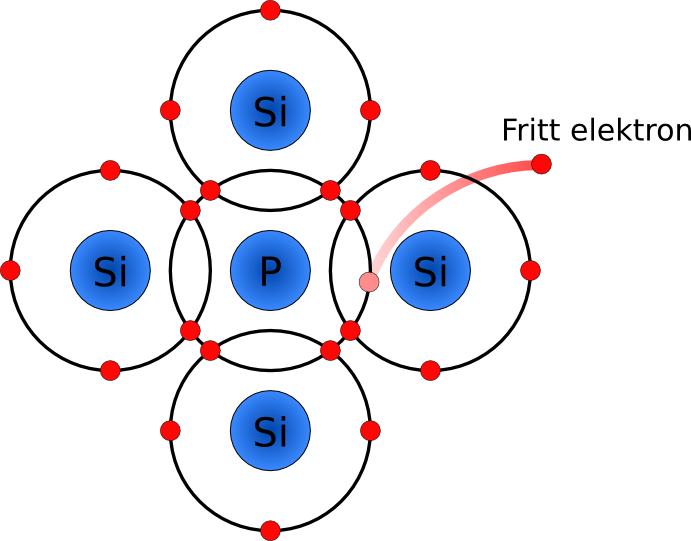
\includegraphics[width=0.5\textwidth]{./img/ntype}
\\
Fosfor blandt silisium.



\subsubsection{p-type}
Akseptor-atomer med 3 valenselektroner
gjør at det er "hull" der det skulle være et elektron.
Disse hullene kan "ta imot" elektroner.
\\\\
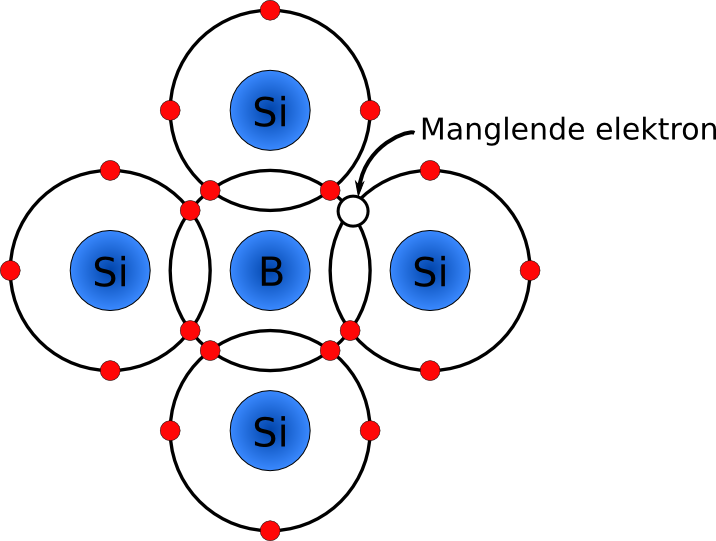
\includegraphics[width=0.5\textwidth]{./img/ptype}
\\
Bor blandt silisium.
